\documentclass[10pt,twocolumn]{article}

\usepackage[T1]{fontenc}
\usepackage[utf8]{inputenc}
\usepackage[margin=0.8in]{geometry}
\usepackage[protrusion=true,expansion=false]{microtype}
\usepackage{graphicx}
\usepackage{booktabs}
\usepackage{tabularx}
\usepackage{amsmath}
\usepackage{amssymb}
\usepackage{enumitem}
\usepackage{xurl}
\usepackage{tikz}
\usepackage{hyperref}
\usepackage[numbers,sort&compress]{natbib}

\usetikzlibrary{arrows.meta,positioning,calc}

\setlength{\columnsep}{0.22in}
\setlength{\tabcolsep}{5pt}
\setlength{\emergencystretch}{3em}
\renewcommand{\arraystretch}{1.08}

\hypersetup{
  colorlinks=true,
  linkcolor=blue,
  citecolor=blue,
  urlcolor=blue
}

\newcommand{\system}{KeelNet}
\newcommand{\abstain}{\textsc{abstain}}

\title{\system: An Extended Summary of Controlled Abstention for Evidence-Grounded Question Answering}
\author{
  Naufal M. Kamaruddin \and
  Ideun Jeong \and
  Author 3
}
\date{\today}

\begin{document}

\maketitle

\begin{abstract}
\system\ studies a narrow version of hallucination control: evidence-grounded
extractive question answering with an explicit answer-or-\abstain\ decision.
Using SQuAD~2.0 \citep{rajpurkar2018know}, the project compares a staged modular
pipeline against several direct-learning alternatives.
The modular path establishes four useful results: abstention supervision
substantially reduces unsupported answers, support verification is learnable,
temperature scaling improves both QA and support calibration, and a calibrated
controller can satisfy the unsupported-answer budget on validation.
The direct-learning and hybrid path establishes four useful negative results: a
support-constrained learner recovers answerable-question quality but becomes too
permissive, an adaptive revision changes the trade-off only weakly, and a
risk-budgeted action learner satisfies validation budgets without carrying that
safety gain to the development split, while the cleaned Stage 8.2 action
learner repeats the same pattern on a truly untouched test split.
The final comparison shows that Stage 5--8.2 recover higher answerable
\(F_1\), but the strongest executed overall groundedness trade-off still comes
from Stage 4 fixed control, and no executed checkpoint reaches the nominal
20\% unsupported-answer budget on the development frontier.
\end{abstract}

\section{Problem and Goal}
\system\ addresses evidence-grounded QA with a constrained action space:
\begin{equation}
f(q, e) \rightarrow \{\text{answer span}, \abstain\},
\end{equation}
where \(q\) is a question and \(e\) is a single evidence passage.
The goal is not to maximize answer extraction alone, but to improve the final
decision trade-off among answer quality, unsupported answering, and abstention.

This framing is intentionally narrower than open-domain hallucination control.
The setup excludes retrieval, multi-hop reasoning, and long-form generation so
that the central question is clean: can a QA system learn when to answer and
when to refuse, while staying tied to the supplied evidence?
That question is closely related to selective prediction and calibration
\citep{geifman2019selectivenet,jiang2021how}, but here it is instantiated in a
single-passage extractive QA setting with explicit unsupported-answer tracking.

\section{Stage Design}
The project proceeds through a staged comparison rather than one monolithic
method.

\begin{enumerate}[leftmargin=1.25em]
  \item \textbf{Stage 1} compares an answer-only baseline against an
  abstain-aware model.
  \item \textbf{Stage 2} adds a support verifier over question, passage, and
  predicted answer.
  \item \textbf{Stage 2.5} retrains the verifier with QA-derived hard
  negatives.
  \item \textbf{Stage 3} calibrates the QA decision score and support score
  with scalar temperature scaling.
  \item \textbf{Stage 4} applies a fixed controller over calibrated QA and
  support signals under an unsupported-answer budget.
  \item \textbf{Stage 5} replaces the modular pipeline with a jointly trained
  support-constrained learner.
  \item \textbf{Stage 6} adds an adaptive balancing layer on top of Stage 5.
  \item \textbf{Stage 7} treats candidate answers and \abstain\ as a shared
  action space with separate utility and risk signals.
  \item \textbf{Stage 8} restores calibrated Stage 4 control on top of the
  frozen Stage 5 answer engine.
  \item \textbf{Stage 8.2} keeps the frozen Stage 5 answer engine but injects
  calibrated Stage 4 support into the Stage 7 action learner and reports its
  final result on a clean final split.
\end{enumerate}

The key experimental question is whether changing the learning objective beats
post-hoc modular control under matched data, backbone, and evaluation
conditions.

\section{Experimental Protocol}
All reported results use SQuAD~2.0 with deterministic train, validation, and
development splits.
The core evaluation metrics are answerable \(F_1\), decision-aware overall
\(F_1\), unsupported-answer rate, and abstain \(F_1\).
Support-aware stages also report answer rate and supported-answer rate among
answered predictions.

The QA backbone is DistilBERT, and later stages keep the same core encoder
family while changing decision logic rather than scaling model size.
The modular path was executed through Stage 4, and the direct-learning path was
executed through Stage 8.2.

\section{Final Learned Architecture}
The final chosen learned architecture is Stage 8.2: a compact decision network
on top of a frozen QA proposal model.
The Stage 5 DistilBERT checkpoint produces a top-\(K\) candidate set
\(\{a_1,\dots,a_K\}\), and the controller adds the explicit abstain action
\(\varnothing\).
Each candidate is described by a 12-dimensional feature vector containing span
quality, calibrated support, abstention, rank, and overlap cues:
\begin{equation}
  x_k =
  [s_{\mathrm{span}}, \Delta_{\mathrm{best}}, \Delta_{\mathrm{next}},
   p_{\mathrm{keep}}, p_{\mathrm{sup}}^{\mathrm{cal}},
   p_{\varnothing}, p_{\mathrm{stage6}}, \ell, r, o, \delta, u].
\end{equation}
The final controller then applies a shallow MLP:
\begin{align}
  h_k &= \mathrm{MLP}(x_k), \\
  u_k &= w_u^\top h_k + b_u, \\
  r_k &= \sigma(w_r^\top h_k + b_r),
\end{align}
where \(u_k\) is the utility logit for answering with candidate \(a_k\) and
\(r_k\) is the predicted unsupported-answer risk.
Abstention is not a thresholded afterthought.
The model pools the candidate states with mean and max pooling and predicts a
separate abstain logit:
\begin{equation}
  u_{\varnothing}
  =
  f_{\mathrm{abs}}([\mathrm{mean}(h_1,\dots,h_K);
  \mathrm{max}(h_1,\dots,h_K)]).
\end{equation}
The final action scores are
\begin{equation}
  s_k = u_k - \lambda_{\mathrm{u}} r_k,
  \qquad
  s_{\varnothing} = u_{\varnothing} - \lambda_{\mathrm{a}},
\end{equation}
followed by softmax over
\([s_1,\dots,s_K,s_{\varnothing}]\).
At inference time, a hard calibrated-support shield can still suppress
candidates whose Stage 4 support probability falls below the selected floor.
So the architecture is hybrid in the deepest sense:
transformer QA proposals, calibrated verifier support, and a small learned
action layer with explicit utility, risk, and abstain heads.

\begin{figure*}[t]
  \centering
  \resizebox{0.98\textwidth}{!}{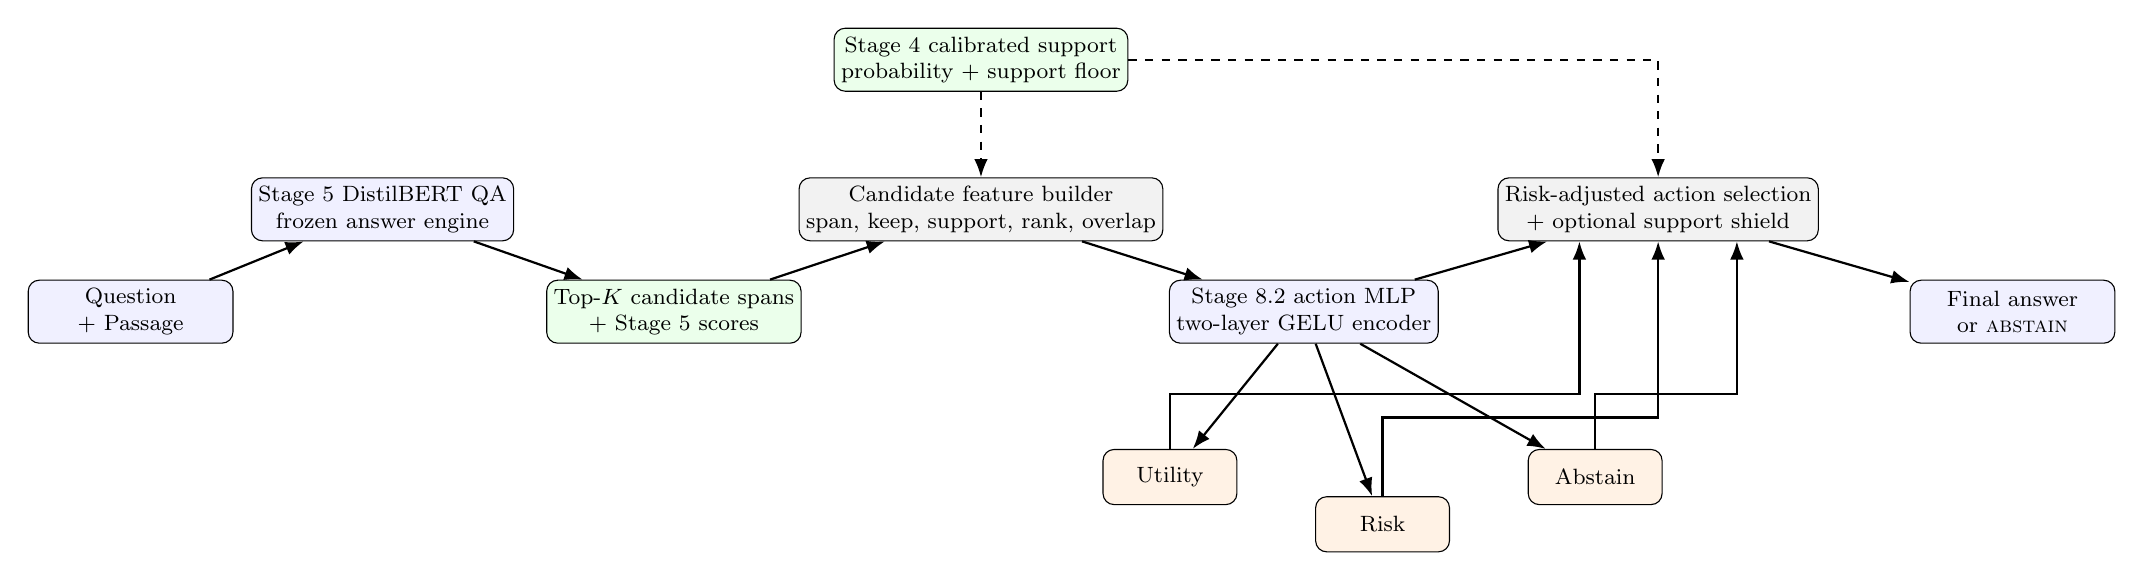
\begin{tikzpicture}[
  >=Latex,
  x=1mm,
  y=1mm,
  every node/.style={font=\footnotesize, align=center},
  block/.style={
    draw,
    rounded corners,
    fill=blue!6,
    minimum width=26mm,
    minimum height=8mm,
    inner sep=2.5pt
  },
  data/.style={
    draw,
    rounded corners,
    fill=green!8,
    minimum width=24mm,
    minimum height=8mm,
    inner sep=2.5pt
  },
  head/.style={
    draw,
    rounded corners,
    fill=orange!10,
    minimum width=17mm,
    minimum height=7mm,
    inner sep=2pt
  },
  merge/.style={
    draw,
    rounded corners,
    fill=gray!10,
    minimum width=31mm,
    minimum height=8mm,
    inner sep=2.5pt
  },
  arrow/.style={->, thick},
  shield/.style={->, thick, dashed}
]

\node[block] (input) at (0,2) {Question\\+ Passage};
\node[block] (stage5) at (32,15) {Stage 5 DistilBERT QA\\frozen answer engine};
\node[data] (cand) at (69,2) {Top-$K$ candidate spans\\+ Stage 5 scores};
\node[merge] (features) at (108,15) {Candidate feature builder\\span, keep, support, rank, overlap};
\node[block] (mlp) at (149,2) {Stage 8.2 action MLP\\two-layer GELU encoder};
\node[merge] (select) at (194,15) {Risk-adjusted action selection\\+ optional support shield};
\node[block] (output) at (239,2) {Final answer\\or \abstain};

\node[data] (support) at (108,34) {Stage 4 calibrated support\\probability + support floor};
\node[head] (utility) at (132,-19) {Utility};
\node[head] (risk) at (159,-25) {Risk};
\node[head] (abstain) at (186,-19) {Abstain};

\draw[arrow] (input) -- (stage5);
\draw[arrow] (stage5) -- (cand);
\draw[arrow] (cand) -- (features);
\draw[arrow] (features) -- (mlp);
\draw[arrow] (mlp) -- (select);
\draw[arrow] (select) -- (output);

\draw[arrow] (mlp) -- (utility);
\draw[arrow] (mlp) -- (risk);
\draw[arrow] (mlp) -- (abstain);
\draw[arrow] (utility.north) -- ++(0,7) -| ([xshift=-10mm]select.south);
\draw[arrow] (risk.north) -- ++(0,10) -| (select.south);
\draw[arrow] (abstain.north) -- ++(0,7) -| ([xshift=10mm]select.south);
\draw[shield] (support) -- (features);
\draw[shield] (support.east) -| (select.north);

\end{tikzpicture}
}
  \caption{Compact left-to-right Stage 8.2 flowchart.
  Frozen Stage 5 QA generates the candidate spans, calibrated Stage 4 support
  enriches and filters them, and a small action network predicts utility,
  risk, and abstain scores before the final answer-or-\abstain\ choice.}
  \label{fig:summary-stage8-2-architecture}
\end{figure*}

\begin{table*}[t]
  \centering
  \caption{Executed checkpoints in the final comparison.
  Most rows report held-out development results; Stage 8.2 reports its clean
  final result on the untouched test split.
  Stage 3 is omitted because it recalibrates scores rather than defining a new
  end-to-end answer-or-\abstain\ system.
  Higher is better for answerable \(F_1\) and overall \(F_1\); lower is better
  for unsupported-answer rate.}
  \label{tab:summary-results}
  \small
  \begin{tabular}{@{}llccc@{}}
    \toprule
    System & Split & Answerable \(F_1\) & Overall \(F_1\) & Unsupported Rate \\
    \midrule
    Stage 1 baseline & dev & 84.82 & 42.35 & 100.00 \\
    Stage 1 abstain-aware & dev & 66.76 & 69.40 & 27.97 \\
    Stage 2 gated QA & dev & 66.41 & 69.42 & 27.57 \\
    Stage 2.5 hard-negative gated QA & dev & 65.62 & 69.34 & 26.95 \\
    Stage 4 fixed controller & dev & 66.41 & 69.41 & 27.59 \\
    Stage 5 support-constrained learner & dev & 71.40 & 68.28 & 34.84 \\
    Stage 6 adaptive learner & dev & 69.70 & 67.62 & 34.45 \\
    Stage 7 action learner & dev & 69.95 & 67.66 & 34.62 \\
    Stage 8 hybrid controller & dev & 68.39 & 68.27 & 31.86 \\
    Stage 8.2 action + calibrated support & test & 70.06 & 68.16 & 33.73 \\
    \bottomrule
  \end{tabular}
\end{table*}

\begin{figure*}[t]
  \centering
  \begin{minipage}[t]{0.54\textwidth}
    \centering
    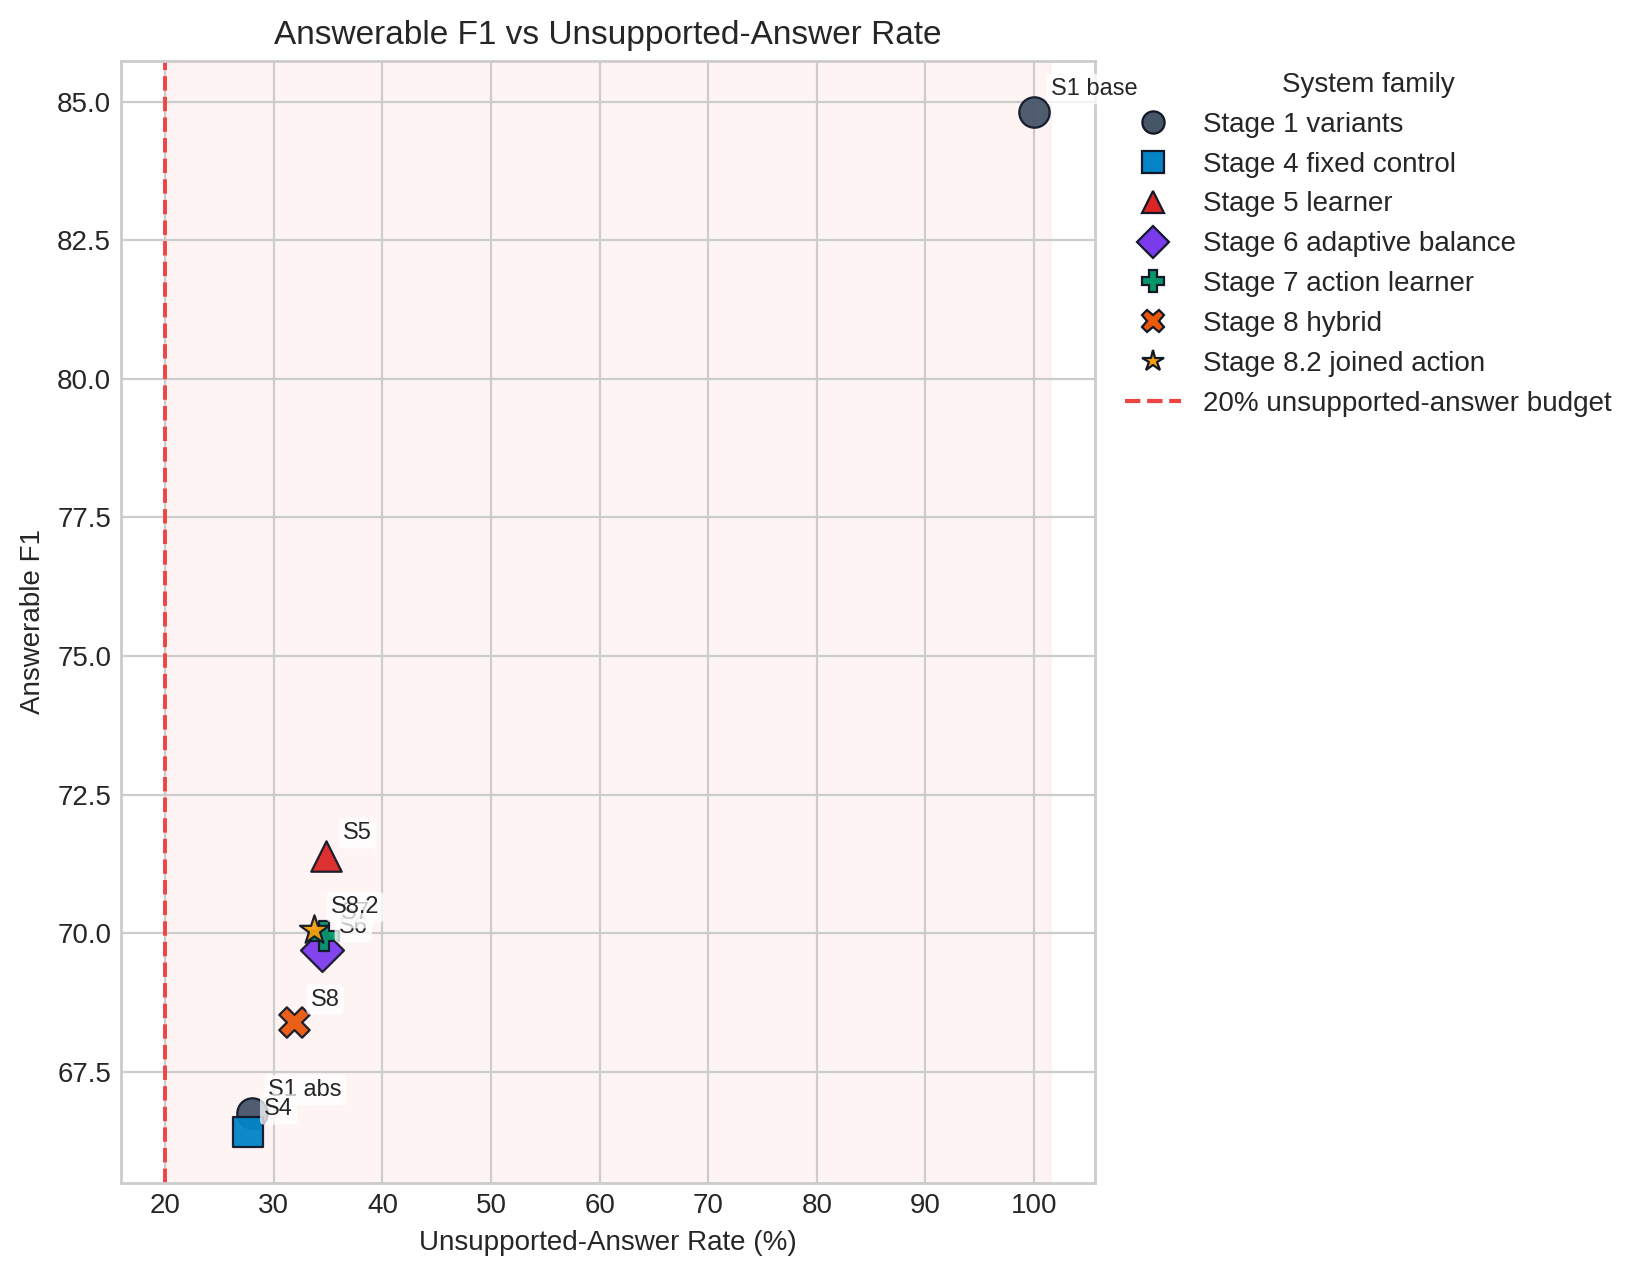
\includegraphics[width=\linewidth]{figures/final-comparison-answerable-f1-vs-unsupported-answer-rate.png}
  \end{minipage}\hfill
  \begin{minipage}[t]{0.42\textwidth}
    \centering
    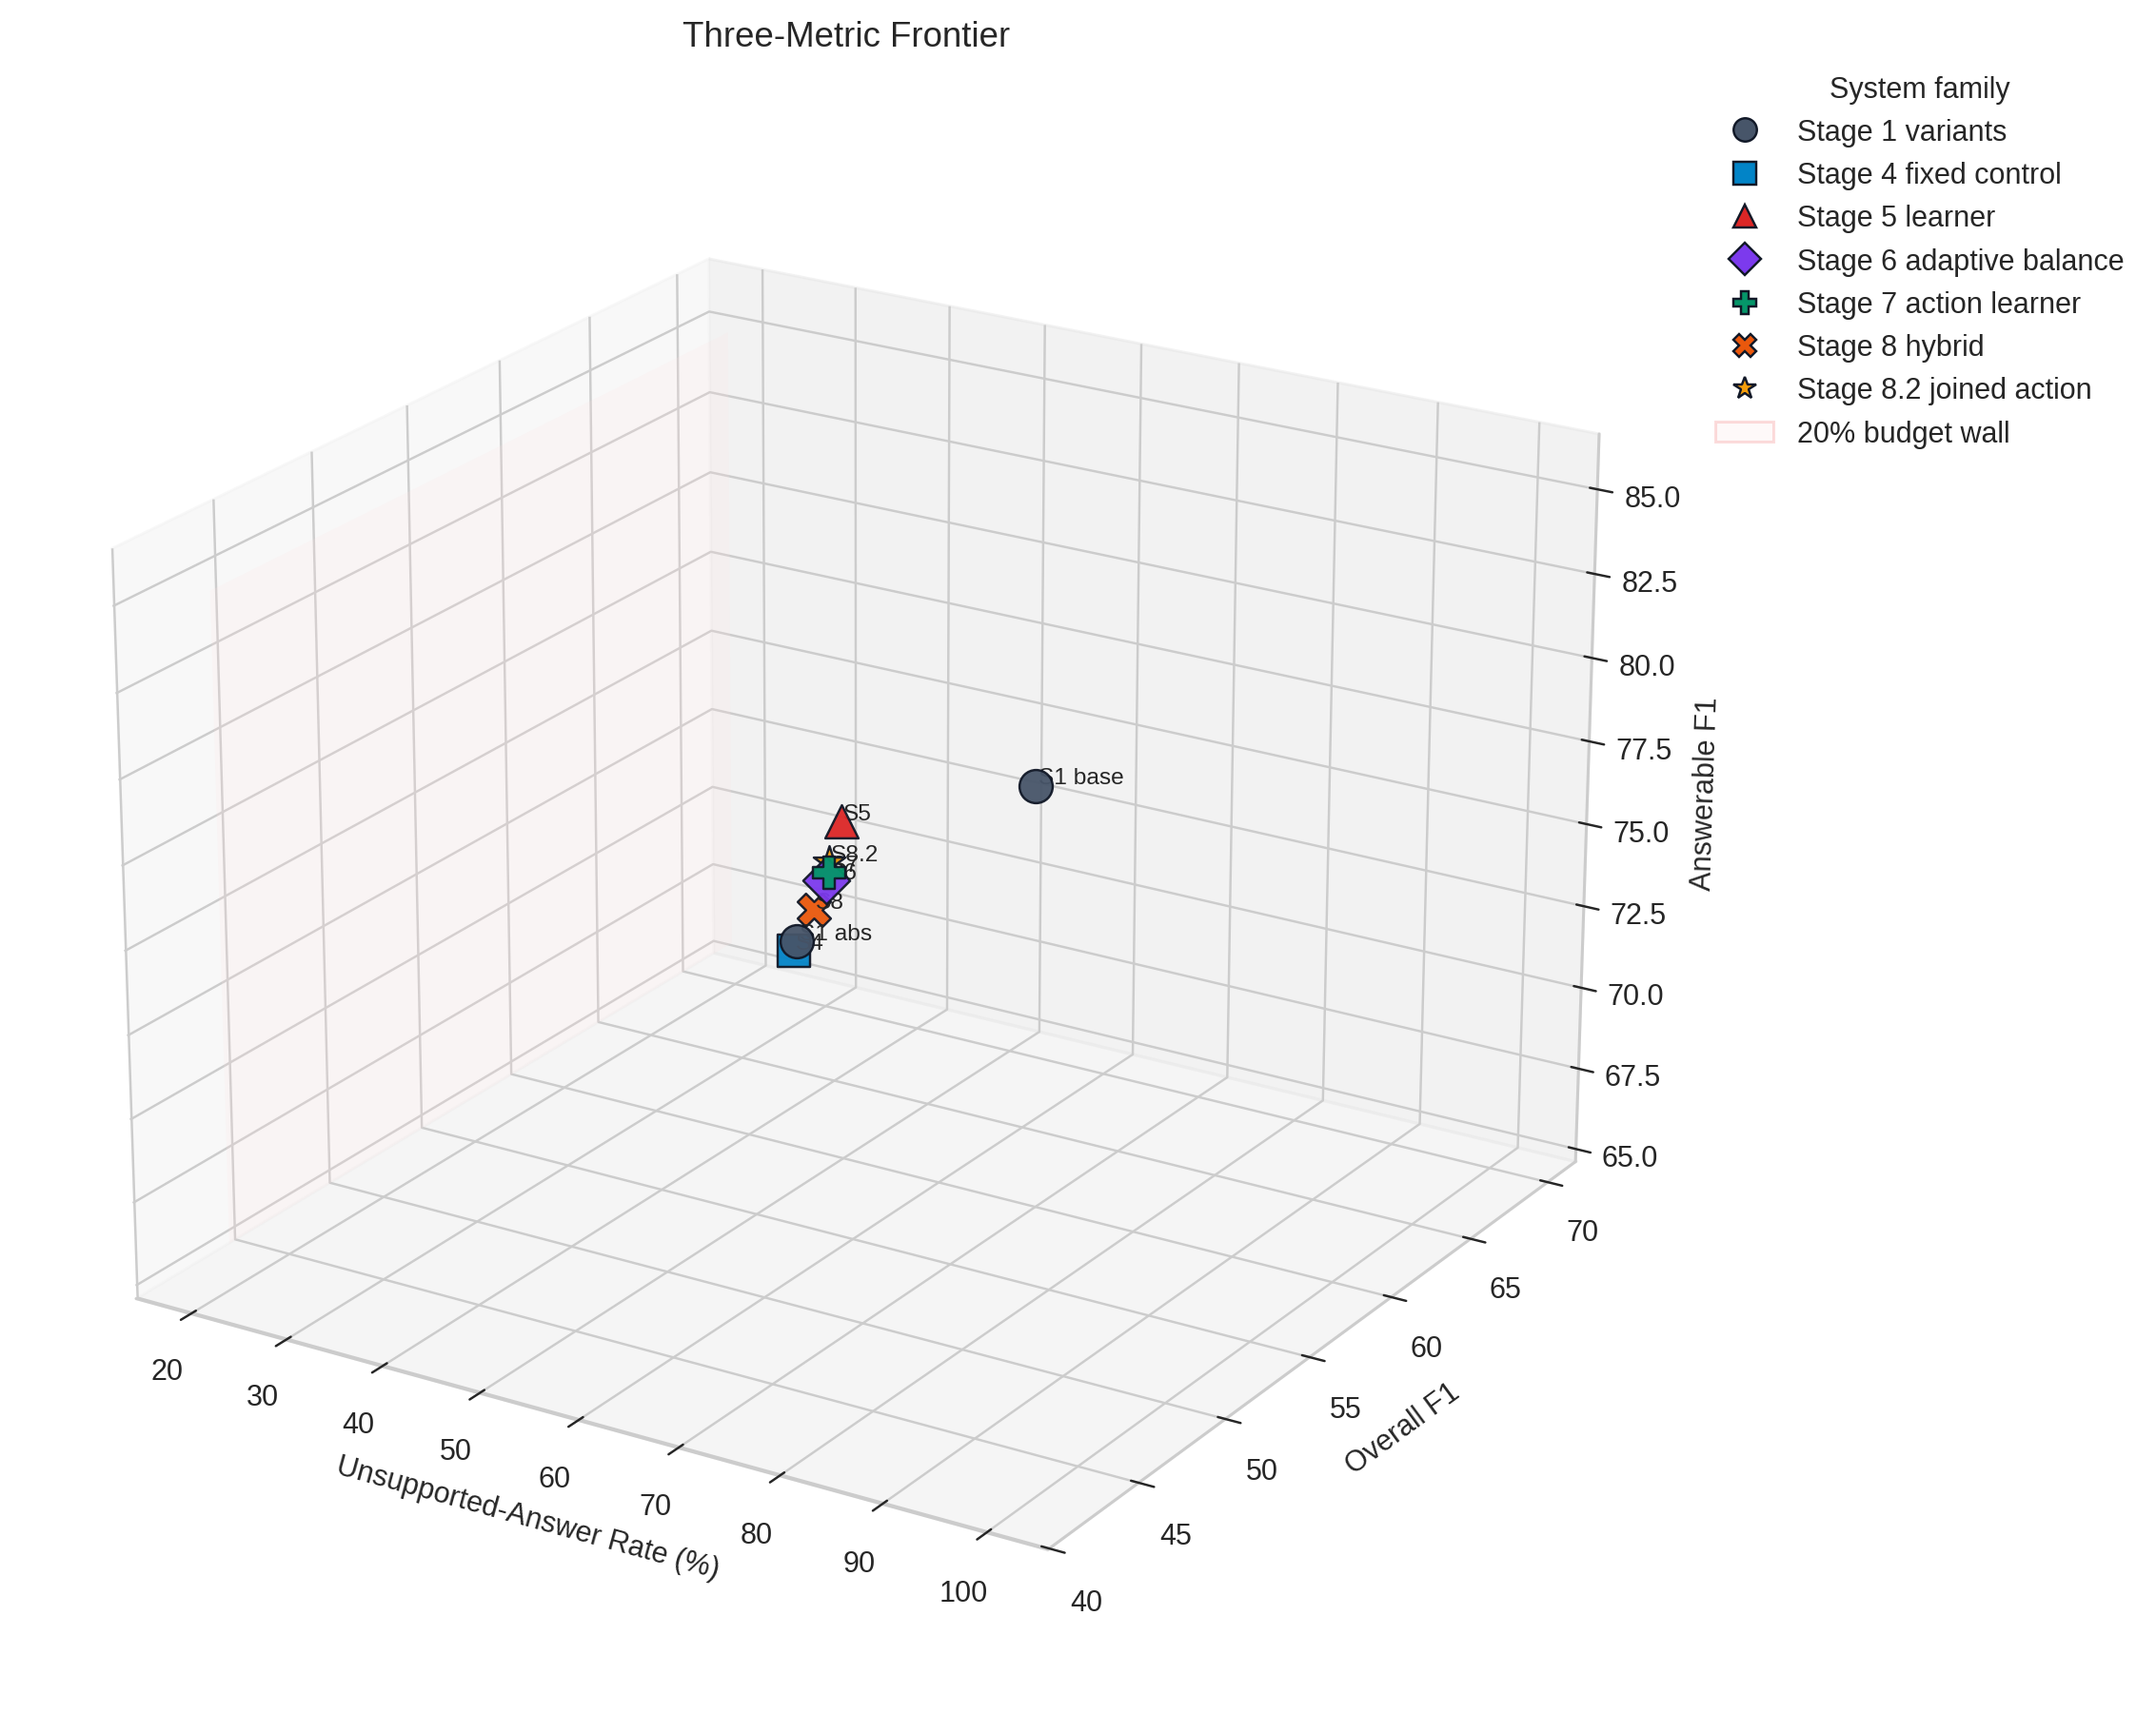
\includegraphics[width=\linewidth]{figures/final-comparison-three-metric-frontier-3d.png}
  \end{minipage}
  \caption{Notebook-generated final comparison frontier.
  The left panel makes the answerable-quality-versus-groundedness trade-off
  explicit: the learned family climbs higher on answerable \(F_1\), but only
  by moving right into a riskier unsupported-answer regime.
  The starred Stage 8.2 point is a clean-split test reference.
  The 3D view makes the same point jointly over unsupported-answer rate,
  overall \(F_1\), and answerable \(F_1\).}
  \label{fig:summary-frontier}
\end{figure*}

\section{Main Findings}
\paragraph{1. Abstention supervision works, but not for free.}
Stage 1 changes the baseline from pathological always-answer behavior into a
meaningful abstention policy.
Unsupported-answer rate drops from 100.00\% to 27.97\%, and overall
\(F_1\) rises from 42.35 to 69.40.
The cost is substantial: answerable \(F_1\) falls from 84.82 to 66.76.
So abstention is learnable, but it introduces a real usefulness-versus-caution
trade-off.

\paragraph{2. Support is learnable, but the verifier remains too permissive.}
Stage 2 shows that support verification is not random noise.
The verifier reaches strong support \(F_1\), but the downstream gated QA system
changes end-to-end behavior only marginally.
Stage 2.5 sharpens this diagnosis.
Hard negatives make the verifier slightly less permissive, lowering dev
unsupported-answer rate from 27.57\% to 26.95\%, but they also lower
answerable \(F_1\) and overall \(F_1\).
This means the verifier-side bottleneck is real, but not removable by a simple
data repair alone.

\paragraph{3. Calibration improves the control signals, especially for QA.}
Stage 3 confirms that both QA and support scores are strongly overconfident.
QA expected calibration error falls from 0.2456 to 0.0753 after temperature
scaling, while support ECE falls from 0.3326 to 0.1708.
This matters because later controller stages depend on score quality rather
than only raw accuracy.
However, support remains the weaker signal even after calibration, which
foreshadows the limits of later controller and learner stages.

\paragraph{4. The first calibrated controller is validation-feasible but
development-flat.}
Stage 4 satisfies the nominal 20\% unsupported-answer budget on validation with
14.30\% unsupported-answer rate and 72.43 overall \(F_1\).
That is a meaningful proof that the calibrated scores can support a constrained
selection policy.
But on development, Stage 4 is effectively a null result relative to Stage 2:
69.41 overall \(F_1\) versus 69.42, and 27.59\% unsupported-answer rate versus
27.57\%.
So calibration improves score quality, but the first fixed controller still
does not leverage those better scores into a better held-out decision rule.

\paragraph{5. Direct learning recovers answer quality faster than it recovers
groundedness.}
Stage 5 is the clearest positive signal for the direct-learning path.
It raises answerable \(F_1\) to 71.40, the best executed result in the later
Stage 1/4/5/6/7 comparison.
But it does so by becoming much more permissive:
unsupported-answer rate rises to 34.84\% and overall \(F_1\) falls to 68.28.
This is a useful negative result, because it reveals the actual failure mode of
the first support-constrained objective:
answer extraction improves faster than unsupported-answer control.

\paragraph{6. The first adaptive, action-based, and hybrid revisions are
informative but still not wins.}
Stage 6 lowers unsupported-answer rate only slightly, from 34.84\% to 34.45\%,
while giving back both answerable \(F_1\) and overall \(F_1\).
Stage 7 is more ambitious.
It satisfies both unsupported-answer and over-abstention budgets on validation,
which is the strongest validation-time safety result in the project.
Yet on development it still reaches 34.62\% unsupported-answer rate, with
67.66 overall \(F_1\).
Stage 8 Hybrid partially recovers groundedness, reaching 68.27 overall \(F_1\)
and 31.86\% unsupported-answer rate on development, but it still does not
recover the Stage 4 modular frontier.
The clean-split Stage 8.2 variant sharpens the same diagnosis:
it satisfies the 20\% unsupported-answer budget on validation with 19.31\%
unsupported-answer rate, then falls back to 33.73\% unsupported-answer rate
and 68.16 overall \(F_1\) on the untouched test split.
So the current bottleneck is no longer just missing action structure or missing
budgets.
It is learning a risk signal whose supported-versus-unsupported separation
generalizes beyond validation.

\paragraph{7. The final comparison shows two distinct regimes rather than one
improving frontier.}
The aggregated final comparison in Figure~\ref{fig:summary-frontier} makes the
overall picture especially clear.
On the answerable-\(F_1\)-versus-unsupported plot, the modular checkpoints sit
around 66--67 answerable \(F_1\) with about 27\% unsupported-answer rate.
By contrast, Stage 5--8 Hybrid shift upward to roughly 68--71 answerable
\(F_1\), but only by moving right into the 32--35\% unsupported-answer range.
The clean-split Stage 8.2 test point lands in the same broad learned-model
regime rather than breaking through it.
In other words, the current direct-learning family has moved the system into a
different operating regime, but not yet to a better groundedness frontier.
No executed checkpoint reaches the nominal 20\% unsupported-answer budget on
the held-out development split.

\section{Conclusion}
The project has now established several useful positive results and several
equally useful negative ones.
The positive results are that abstention supervision works, support prediction
is viable, score calibration improves the quality of downstream control
signals, and a validation-feasible calibrated controller can be selected.
The negative results are that verifier repair alone does not remove the modular
bottleneck, the first jointly trained learner is too permissive, the first
adaptive revision is too weak, and neither the risk-budgeted nor the cleaned
hybrid revisions transfer their validation-side safety gains tightly enough to
held-out data.

The final architectural lesson is therefore specific.
If the goal is the best executed operating point today, Stage 4 fixed control
is still the answer.
If the goal is the clearest deep-learning formulation of support-aware answer
selection, Stage 8.2 is the right final model to carry forward:
frozen QA proposals, calibrated support features, and a learned
utility-versus-risk action layer with an explicit abstain head.

The strongest current conclusion is therefore diagnostic rather than triumphant:
the remaining bottleneck is not whether abstention, support, or calibration are
possible at all, but whether the system can learn a risk signal that
generalizes tightly enough to control unsupported answering on held-out data.
That keeps the main research direction alive, but it also changes the standard
for success.
Future work should be judged not by whether it merely changes the trade-off,
but by whether it improves groundedness without collapsing utility on the same
development frontier.

\begingroup
\small
\bibliographystyle{plainnat}
\bibliography{refs}
\endgroup

\end{document}
